\documentclass[11pt]{article}

% Language setting
\usepackage[turkish]{babel}
\usepackage{pythonhighlight}
\usepackage{graphicx}
\usepackage[a4paper,top=2cm,bottom=2cm,left=2cm,right=2cm,marginparwidth=2cm]{geometry}

% Useful packages
\usepackage{amsmath}
\usepackage{graphicx}
\usepackage[colorlinks=true, allcolors=blue]{hyperref}
\usepackage{verbatim}
\usepackage{fancyhdr} % for header and footer
\usepackage{titlesec}
\usepackage{parskip}

\setlength{\parindent}{0pt}

\titleformat{\subsection}[runin]{\bfseries}{\thesubsection}{1em}{}

\pagestyle{fancy} % activate the custom header/footer

% define the header/footer contents
\lhead{\small{23BLM-4014 Yapay Sinir Ağları Ara Sınav Soru ve Cevap Kağıdı}}
\rhead{\small{Dr. Ulya Bayram}}
\lfoot{}
\rfoot{}

% remove header/footer on first page
\fancypagestyle{firstpage}{
  \lhead{}
  \rhead{}
  \lfoot{}
  \rfoot{\thepage}
}
 

\title{Çanakkale Onsekiz Mart Üniversitesi, Mühendislik Fakültesi, Bilgisayar Mühendisliği Akademik Dönem 2022-2023\\
Ders: BLM-4014 Yapay Sinir Ağları/Bahar Dönemi\\ 
ARA SINAV SORU VE CEVAP KAĞIDI\\
Dersi Veren Öğretim Elemanı: Dr. Öğretim Üyesi Ulya Bayram}
\author{%
\begin{minipage}{\textwidth}
\raggedright
Öğrenci Adı Soyadı: Nazlıcan Çay \\ % Adınızı soyadınızı ve öğrenci numaranızı noktaların yerine yazın
Öğrenci No: 190401064
\end{minipage}%
}

\date{14 Nisan 2023}

\begin{document}
\maketitle

\vspace{-.5in}
\section*{Açıklamalar:}
\begin{itemize}
    \item Vizeyi çözüp, üzerinde aynı sorular, sizin cevaplar ve sonuçlar olan versiyonunu bu formatta PDF olarak, Teams üzerinden açtığım assignment kısmına yüklemeniz gerekiyor. Bu bahsi geçen PDF'i oluşturmak için LaTeX kullandıysanız, tex dosyasının da yer aldığı Github linkini de ödevin en başına (aşağı url olarak) eklerseniz bonus 5 Puan! (Tavsiye: Overleaf)
    \item Çözümlerde ya da çözümlerin kontrolünü yapmada internetten faydalanmak, ChatGPT gibi servisleri kullanmak serbest. Fakat, herkesin çözümü kendi emeğinden oluşmak zorunda. Çözümlerinizi, cevaplarınızı aşağıda belirttiğim tarih ve saate kadar kimseyle paylaşmayınız. 
    \item Kopyayı önlemek için Github repository'lerinizin hiçbirini \textbf{14 Nisan 2023, saat 15:00'a kadar halka açık (public) yapmayınız!} (Assignment son yükleme saati 13:00 ama internet bağlantısı sorunları olabilir diye en fazla ekstra 2 saat daha vaktiniz var. \textbf{Fakat 13:00 - 15:00 arası yüklemelerden -5 puan!}
    \item Ek puan almak için sağlayacağınız tüm Github repository'lerini \textbf{en geç 15 Nisan 2023 15:00'da halka açık (public) yapmış olun linklerden puan alabilmek için!}
    \item \textbf{14 Nisan 2023, saat 15:00'dan sonra gönderilen vizeler değerlendirilmeye alınmayacak, vize notu olarak 0 (sıfır) verilecektir!} Son anda internet bağlantısı gibi sebeplerden sıfır almayı önlemek için assignment kısmından ara ara çözümlerinizi yükleyebilirsiniz yedekleme için. Verilen son tarih/saatte (14 Nisan 2023, saat 15:00) sistemdeki en son yüklü PDF geçerli olacak.
    \item Çözümlerin ve kodların size ait ve özgün olup olmadığını kontrol eden bir algoritma kullanılacaktır. Kopya çektiği belirlenen vizeler otomatikman 0 (sıfır) alacaktır. Bu nedenle çözümlerinizi ve kodlarınızı yukarıda sağladığım gün ve saatlere kadar kimseyle paylaşmayınız.
    \item Bu vizeden alınabilecek en yüksek not 100'dür. Toplam aldığınız puan 100'ü geçerse, aldığınız not 100'e sabitlenecektir.
    \item LaTeX kullanarak PDF oluşturanlar öz geçmişlerine LaTeX bildiklerini de eklemeyi unutmasınlar :)
    \item Bu vizedeki soruların çözümleri ve tex dosyası için istediğiniz kadar sayıda Github repository'si oluşturabilirsiniz. Sadece yukarıda belirttiğim tarihlerde (14 Nisan 2023 saat 15:00 ile 15 Nisan 2023 saat 15:00 arasında) public yapmayı/halka açmayı ve Github profilinizi de öz geçmişinize eklemeyi unutmayın :)
    \item Bilgisayarınıza hiçbir program kurmadan, Overleaf, Google Colab, Kaggle gibi ortamlar üzerinden bu vizeyi tamamlamanız mümkün. İyi çalışmalar!!
\end{itemize}

(Ekstra 5 puan) \url{OdevinTexDosyasınınGithubLinkiniburayakoyun.com}

\newpage
\section{(Toplam 10 Puan) Hopfield Networks:}

\subsection{(2 Puan)} \textbf{ChatGPT’ye size Hopfield Network’ler ile ilgili detaylı bilgi vermesini isteyin. Sorduğunuz soruyu, ChatGPT'nin çıkartığı cevabı aşağı koyun. Bu cevapta anlamadığınız terimleri de ChatGPT’ye sorup, sorduğunuz soruları ve ChatGPT’nin verdiği cevapları da sırayla aşağı koyun.}


Elbette! Hopfield ağları, yapay sinir ağı modellerinden biridir ve adını John Hopfield'dan almıştır. 1982'de tanıtılan bu ağ modeli, hafıza ve tanıma yetenekleriyle bilinir. İki temel uygulama alanı, örüntü tanıma ve optimize etme problemleridir.

Hopfield ağları, geri beslemeli bir ağdır ve nöronlar arasındaki bağlantıların güçleri belirli bir matrisle temsil edilir. Bu matris, "öğrenme" sırasında belirlenir ve ağın işlevi buna bağlıdır. Bu matris, nöronların birbirleriyle olan bağlantılarının gücünü belirleyen ve ağın davranışını yönlendiren bir ağırlık matrisidir.

Bir Hopfield ağı, birbirleriyle bağlantılı nöronlardan oluşur ve bu nöronlar genellikle iki durumlu (aktif ve pasif) olarak modellenir. Her nöron, diğer tüm nöronlara bağlıdır ve her bağlantının gücü, o bağlantının ağırlık matrisindeki ilgili eleman tarafından belirlenir. Ağırlık matrisi, ağın hafızasını temsil eder ve öğrenme süreci sırasında belirlenir.

Hopfield ağları, bir örüntüyü hatırlama yeteneği ile tanınır. 
Bir örüntü, nöronların birbirleriyle olan bağlantılarındaki 
ağırlıkların belirli bir şekilde ayarlanmasıyla ağın 
hafızasına kaydedilir. 
Sonra, ağa farklı bir örüntü sunulduğunda, ağ o örüntüyü 
tanıyacak ve kaydedilen örüntüye en yakın olan ö-
 rüntüyü hatırlayacaktır.

Hopfield ağları ayrıca optimize etme problemleri için de kullanılabilir. Örneğin, bir Hopfield ağı kullanarak, belirli bir örüntü seti için minimum enerjiyi sağlayacak şekilde ağırlıkları ayarlayabilirsiniz.

Hopfield ağları, yapay zeka, örüntü tanıma, veri sıkıştırma, optimize etme problemleri ve bellek modellemesi gibi birçok alanda kullanılmaktadır.

\underline{Geri Beslemeli ağlar : } Geri beslemeli ağlar, bir çıktının tekrar girdi olarak kullanıldığı, çıkışın kendisine bir geri besleme döngüsü oluşturduğu bir yapay sinir ağı türüdür. Bu tür ağlar, gerçek dünyadaki birçok sistemde gözlemlenebilen geri besleme döngüleri ile benzerlik gösterirler.

Geri beslemeli ağlar, ileri beslemeli ağlardan farklı olarak, çıktıları girdi olarak kullanarak kendi davranışlarını etkileyebilirler. Bu sayede, önceki girdilere göre daha uygun sonuçlar üretme yeteneği kazanırlar.




\
\
\ 

\subsection{(8 Puan)} \textbf{ChatGPT’nin açıklamalarından ne anladığınızı buraya kendi kelimelerinizle özetleyin. Örneğin ``Hopfield Network nedir? Ne işe yarar? Neden bilmemiz gerekir bunu? Gerçek hayatta kullanılıyor mu?'' gibi. Anlamadığınız kısımlar varsa ve ChatGPT’nin açıklamaları yeterli gelmezse internet dahil farklı kaynaklardan araştırıp, bilgilerin doğruluğunu sorgulamakta serbestsiniz. Konuyu doğru anlayıp anlamamanız puana etki edecektir. Kullandığınız kaynakları da belirtin!}

Hopfield Networkleri hafıza vetanıma özelliklerine sahip, geri beslemeli bir ağdır. Hopfield networkleri öğrenme yetisine sahiptir. Birbirleriyle bağlantılı nörönlardan oluşur. Nörönlar arasındaki bağlar ögrenme gerçekleşirken güçlenir. 
Öğrenme yetileri sayesinde Hopfield Networklerine örüntüler öğretilebilir. Öğrendiği örüntüler hafızasına kaydedilir. 
Bu sayedec ilerde başka bir örüntü ağa verildiğinde öğrendiği örüntüler arasından en benzer örüntüyü bize verir. Günlük hayatta bu ögrenme ve benzerini cıktı verme özelliği kullanılabileceği gibi optimizasyon problemlerinde de kullanılır . 

\section{(Toplam 10 Puan) Boltzman Machine:}

\subsection{(2 Puan)} \textbf{ChatGPT’ye size Boltzman Machine ilgili detaylı bilgi vermesini isteyin. Sorduğunuz soruyu, ChatGPT'nin çıkartığı cevabı aşağı koyun. Bu cevapta anlamadığınız terimleri de ChatGPT’ye sorup, sorduğunuz soruları ve ChatGPT’nin verdiği cevapları da sırayla aşağı koyun.}

Boltzmann Machine, öğrenme ve örüntü tanıma problemlerini çözmek için kullanılan, enerji işlemi prensibine dayanan bir tür yapay sinir ağıdır. Bu ağ, adını fizikçi Ludwig Boltzmann'dan alır ve ilk olarak 1980'lerde keşfedilmiştir.

Bir Boltzmann Machine, nöronları (sinir hücreleri) ve bağlantıları içeren bir ağdır. Her nöron, bir aktivasyon durumu (açık veya kapalı) ve bir eşik değeri (threshold) taşır. Aynı şekilde, her bağlantı ağırlığı da bir sayısal değer ile ifade edilir.

Bir Boltzmann Machine'in işleyişi, bir enerji fonksiyonu veya maliyet fonksiyonu kullanarak hesaplanır. Bu fonksiyon, nöronların aktivasyon durumlarına ve bağlantıların ağırlıklarına bağlı olarak bir enerji seviyesi hesaplar. Daha düşük bir enerji seviyesi, daha istenen bir durumu ifade eder.

Bir Boltzmann Machine, bir veri kümesindeki örüntüleri tanımak için eğitilebilir. Eğitim sırasında, ağın her bir nöronu, ağırlık ve eşik değerlerinin optimize edilmesi için yeniden hesaplanır. Bu işlem, maksimum olasılık öğrenmesi (maximum likelihood learning) olarak bilinir ve Stokastik Gradient İniş (Stochastic Gradient Descent) gibi optimizasyon teknikleri ile gerçekleştirilir.

Bir Boltzmann Machine'in en önemli özelliklerinden biri, giriş verilerinin eksiksiz olması gerekmeyişidir. Ağ, giriş verilerinin tamamını veya bir kısmını alabilir ve ardından eksik verileri tamamlayabilir.

Boltzmann Machine'ler, özellikle veri sıkıştırma, örüntü tanıma, doğal dil işleme, öneri sistemleri, robotik ve görüntü işleme gibi alanlarda kullanılmaktadır. Ancak, eğitim süreleri uzun ve ağların karmaşıklığı nedeniyle hesaplama maliyetleri yüksek olabilir. Bu nedenle, son yıllarda daha hızlı ve daha ölçeklenebilir yapay sinir ağlarına odaklanılmıştır.

\underline{Maximum likelihood learning : } Maximum likelihood learning, Boltzmann Machine ve diğer birçok öğrenme algoritmasının temelinde yatan bir prensiptir. Bu prensip, bir veri kümesindeki örüntüleri tanımak ve modellemek için kullanılır.

Bir Boltzmann Machine'in eğitimi sırasında, ağın her bir nöronu için, veri kümesindeki örüntülerin olasılığı hesaplanır. Bu olasılık, nöronun aktivasyon durumuna ve ağdaki diğer nöronların aktivasyon durumlarına bağlıdır. Modelin maksimum olasılığı bulunmaya çalışılır ve bunun için ağırlık ve eşik değerleri optimize edilir.

\underline{Stokastik gradient iniş : } Stokastik gradient iniş, ağın eğitiminde sıklıkla kullanılan bir optimizasyon algoritmasıdır. Bu algoritma, her bir eğitim örneği için gradyan hesaplar ve gradyanın yönünde ağırlık ve eşik değerlerini günceller. Bu işlem, ağırlıkları en iyi sonuç veren değerlere yaklaştırmaya yardımcı olur.

Stokastik gradient iniş, ağın eğitim süresini kısaltır ve hesaplama maliyetlerini düşürür. Bu nedenle, büyük veri setleri üzerinde eğitim yaparken sıklıkla tercih edilir.


\subsection{(8 Puan)} \textbf{ChatGPT’nin açıklamalarından ne anladığınızı buraya kendi kelimelerinizle özetleyin. Örneğin ``Boltzman Machine nedir? Ne işe yarar? Neden bilmemiz gerekir bunu? Gerçek hayatta kullanılıyor mu?'' gibi. Anlamadığınız kısımlar varsa ve ChatGPT’nin açıklamaları yeterli gelmezse internet dahil farklı kaynaklardan araştırıp, bilgilerin doğruluğunu sorgulamakta serbestsiniz. Konuyu doğru anlayıp anlamamanız puana etki edecektir. Kullandığınız kaynakları da belirtin!}

Boltzman Machine de hopfield Networkleri gibi enerji fonksiyonu tabanlı ve geri beslemeli bir sinir ağı modelleridir. Herbir bir aktivasyon durumuna sahip nörönlardan oluşan bir ağa sahiptir. işleyişi hesaplanırken bir maliyet veya enerji fonksiyonundan yaralanılır. Boltzman Machine unsupervised learning de yaygın kullanılır. Günlük hayatta Görüntü tanıma, Doğal Dil İşleme ve Öneri sistemleri gibi projelerde kullanılabilir.


\section{(Toplam 10 Puan) Markov Assumption ve Markov Chain:}

\subsection{(2 Puan)} \textbf{ChatGPT’ye size Markov assumption ve Markov Chain ilgili detaylı bilgi vermesini isteyin. Sorduğunuz soruyu, ChatGPT'nin çıkartığı cevabı aşağı koyun. Bu cevapta anlamadığınız terimleri de ChatGPT’ye sorup, sorduğunuz soruları ve ChatGPT’nin verdiği cevapları da sırayla aşağı koyun.}

Markov Assumption ve Markov Chain, istatistiksel ve olasılık teorisi alanında önemli kavramlardır. İşte her biri hakkında daha detaylı bilgi:

Markov Assumption:
Markov Assumption, bir olayın yalnızca anlık durumunun, geçmişteki durumlarından bağımsız olduğunu varsayar. Yani, bir sonraki durum yalnızca mevcut durumdan etkilenir ve tüm önceki durumlarla ilgili bilgi yok sayılır. Bu varsayım, "Markov Özelliği" olarak da bilinir.

Markov Chain:
Markov Chain, bir dizi durumun birbirini takip ettiği, her bir durumun yalnızca mevcut duruma bağlı olduğu bir modeldir. Markov Chain, belirli bir olasılık dağılımı kullanarak herhangi bir iki durum arasındaki olasılık ilişkisini modeller. Markov Chain, belirli bir durumdan başlayarak rastgele bir şekilde ilerleyerek son duruma ulaşan, ayrık zamanlı bir süreçtir.

Markov Chain'in temel bileşenleri:

Durumlar: Markov Chain'de birbirini takip eden durumlar mevcuttur. Örneğin, bir zar atışında durumlar 1, 2, 3, 4, 5 ve 6'dır.
Geçiş olasılıkları: Bir durumdan diğer bir duruma geçiş olasılıkları, Markov Chain'deki temel olasılık bileşenleridir. Örneğin, bir zar atışında, bir durumdan diğerine geçiş olasılığı 1/6'dır.
Başlangıç olasılıkları: Markov Chain'in başlangıç durumları, bir başlangıç olasılığı dağılımı ile modellenir.
Durum dağılımı: Markov Chain'de, herhangi bir anda sistemin bulunduğu durumların olasılık dağılımı, durum dağılımı olarak bilinir.
Markov Chain, birçok alanda kullanılan bir modeldir. Örneğin, ekonomi, finans, mühendislik, fizik, biyoloji, bilgisayar bilimleri ve yapay zeka gibi birçok alanda kullanılır. Markov Chain, zaman içinde değişen bir sistemdeki davranışı modellerken, Markov Assumption ise sistem davranışının yalnızca anlık durumdan etkilendiğini varsayar.

\underline{Markov assamption in de temel bileşenleri var mı varsa neler : }
\ 

Markov Assumption'un temel bileşenleri şunlardır:

Durumlar: Markov Assumption, bir olayın yalnızca anlık durumunun, geçmişteki durumlarından bağımsız olduğunu varsayar. Bu nedenle, her bir durum bu anlık durumu ifade eder.
Geçiş olasılıkları: Markov Assumption, bir sonraki durumun yalnızca mevcut durumdan etkilendiğini varsayar. Bu nedenle, bir durumdan diğerine geçiş olasılıkları, yalnızca mevcut durumun bilgisine dayanır.
Başlangıç durumu: Markov Assumption, herhangi bir olayın başlangıç durumunu varsayar. Başlangıç durumu, bir sonraki durumu belirlemede önemlidir.
Markov Assumption, özellikle zaman serileri ve sinyal işleme gibi zamanla değişen verilerin analizi için yaygın olarak kullanılır. Bu varsayım, verilerin modellemesi için özellikle kullanışlıdır, çünkü gelecekteki durumların mevcut duruma bağlı olduğu durumlarda yüksek doğrulukla sonuçlar üretebilir.


\subsection{(8 Puan)} \textbf{ChatGPT’nin açıklamalarından ne anladığınızı buraya kendi kelimelerinizle özetleyin. Örneğin ``Markov assumption ve Markov Chain nedir? Ne işe yarar? Neden bilmemiz gerekir bunu? Gerçek hayatta kullanılıyor mu?'' gibi. Anlamadığınız kısımlar varsa ve ChatGPT’nin açıklamaları yeterli gelmezse internet dahil farklı kaynaklardan araştırıp, bilgilerin doğruluğunu sorgulamakta serbestsiniz. Konuyu doğru anlayıp anlamamanız puana etki edecektir. Kullandığınız kaynakları da belirtin!}

Markov assumption ve Markov Chain olaılık teorisinde kullanılan temel kavramlardandır.

markov assumption a göre bir olayın gelecekteki durumu yanlızca su anki durumuna bağlıdır. olayın geçmişteki durumlarından bağamsızdır. 

Markov Assumption, özellikle zaman serileri ve sinyal işleme gibi zamanla değişen verilerin analizi için yaygın olarak kullanılır. Bunun yanı sıra, Makine Öğrenmesi, Finansal Piyasalar, İletişim Ağları ve Yapay Zeka alanlarında da kullanılır. 

Markov Chain ise olayın durumlarının zincirleme ilerleğini düşünür. Bir olayın gelecekteki durumu, gecmişteki durumlarından etkilenir bu yüzden bir önceki durum kayıt altında tutulur.

Markov Chain, zaman serileri, rastgele yürüyüşler, kuyruklu sistemler ve doğal dil işleme gibi birçok alanda kullanılır. Ayrıca, Markov Chain'ler, Bayes ağları ve gizli Markov modelleri gibi diğer istatistiksel modellerin oluşturulmasında da kullanılır.


\section{(Toplam 20 Puan) Feed Forward:}
 
\begin{itemize}
    \item Forward propagation için, input olarak şu X matrisini verin (tensöre çevirmeyi unutmayın):\\
    $X = \begin{bmatrix}
        1 & 2 & 3\\
        4 & 5 & 6
        \end{bmatrix}$
    Satırlar veriler (sample'lar), kolonlar öznitelikler (feature'lar).
    \item Bir adet hidden layer olsun ve içinde tanh aktivasyon fonksiyonu olsun
    \item Hidden layer'da 50 nöron olsun
    \item Bir adet output layer olsun, tek nöronu olsun ve içinde sigmoid aktivasyon fonksiyonu olsun
\end{itemize}

Tanh fonksiyonu:\\
$f(x) = \frac{exp(x) - exp(-x)}{exp(x) + exp(-x)}$
\vspace{.2in}

Sigmoid fonksiyonu:\\
$f(x) = \frac{1}{1 + exp(-x)}$

\vspace{.2in}
 \textbf{Pytorch kütüphanesi ile, ama kütüphanenin hazır aktivasyon fonksiyonlarını kullanmadan, formülünü verdiğim iki aktivasyon fonksiyonunun kodunu ikinci haftada yaptığımız gibi kendiniz yazarak bu yapay sinir ağını oluşturun ve aşağıdaki üç soruya cevap verin.}


\clearpage %Page break


\subsection{(10 Puan)} \textbf{Yukarıdaki yapay sinir ağını çalıştırmadan önce pytorch için Seed değerini 1 olarak set edin, kodu aşağıdaki kod bloğuna ve altına da sonucu yapıştırın:}

% Latex'de kod koyabilirsiniz python formatında. Aşağıdaki örnekleri silip içine kendi kodunuzu koyun


\begin{python}
import torch
In [226]:
# X matrisini tanımlayım
X = [[1, 2, 3], [4, 5, 6]]
In [227]:
# X matrisini bir PyTorch Tensor nesnesine dönüştürün
tensor_X = torch.tensor(X)
In [228]:
# Modeli tanımlayın
inputSize = 3
hiddenSize = 50
outputSize = 1

W1 = torch.randn(hiddenSize, inputSize)
b1 = torch.randn(hiddenSize, 1)
W2 = torch.randn(outputSize, hiddenSize)
b2 = torch.randn(outputSize, 1)

#  seed değerini 1 girelim 

torch.manual_seed(1)
# Tanh aktivasyon fonksiyonu
def tanh(x):
     return (torch.exp(x) - torch.exp(-x)) / (torch.exp(x) + torch.exp(-x))
In [230]:
# Sigmoid aktivasyon fonksiyonu
def sigmoid(x):
    return 1 / (1 + torch.exp(-x))
In [231]:
# Forward propagation işlemi
Z1 = torch.matmul(W1, tensor_X.transpose(0, 1).float()) + b1
A1 = tanh(Z1)
Z2 = torch.matmul(W2, A1) + b2
A2 = sigmoid(Z2)
# Sonucu yazdırın
print(A2)

# torch fonksiyonuyla deneyerek cevabın sağlamasını yapalım.

torch.manual_seed(1)
A1 =torch.tanh(A1)
Z2 = torch.matmul(W2, A1) + b2
A2 = torch.sigmoid(Z2)
print(A2)
\end{python}

tensor([[0.0312, 0.0075]])
tensor([[0.0422, 0.0214]])
\clearpage %Page break
\subsection{(5 Puan)} \textbf{Yukarıdaki yapay sinir ağını çalıştırmadan önce Seed değerini öğrenci numaranız olarak değiştirip, kodu aşağıdaki kod bloğuna ve altına da sonucu yapıştırın:}

\begin{python}
import torch
In [219]:
# X matrisini tanımlayım
X = [[1, 2, 3], [4, 5, 6]]
In [220]:
# X matrisini bir PyTorch Tensor nesnesine dönüştürün
tensor_X = torch.tensor(X)
In [221]:
# Modeli tanımlayın
inputSize = 3
hiddenSize = 50
outputSize = 1

W1 = torch.randn(hiddenSize, inputSize)
b1 = torch.randn(hiddenSize, 1)
W2 = torch.randn(outputSize, hiddenSize)
b2 = torch.randn(outputSize, 1)

# custom bir seed değeri girelim 
torch.manual_seed(190401064)
In [222]:
# Tanh aktivasyon fonksiyonu
def tanh(x):
     return (torch.exp(x) - torch.exp(-x)) / (torch.exp(x) + torch.exp(-x))
In [223]:
# Sigmoid aktivasyon fonksiyonu
def sigmoid(x):
    return 1 / (1 + torch.exp(-x))
In [224]:
# Forward propagation işlemi
Z1 = torch.matmul(W1, tensor_X.transpose(0, 1).float()) + b1
A1 = tanh(Z1)
Z2 = torch.matmul(W2, A1) + b2
A2 = sigmoid(Z2)
# Sonucu yazdırın
print(A2)

# torch fonksiyonuyla deneyerek cevabın sağlamasını yapalım.

torch.manual_seed(190401064)
A1 =torch.tanh(A1)
Z2 = torch.matmul(W2, A1) + b2
A2 = torch.sigmoid(Z2)
print(A2)
\end{python}

ensor([[1.0000, 0.9997]])
tensor([[1.0000, 0.9997]])

\subsection{(5 Puan)} \textbf{Kodlarınızın ve sonuçlarınızın olduğu jupyter notebook'un Github repository'sindeki linkini aşağıdaki url kısmının içine yapıştırın. İlk sayfada belirttiğim gün ve saate kadar halka açık (public) olmasın:}
% size ait Github olmak zorunda, bu vize için ayrı bir github repository'si açıp notebook'u onun içine koyun. Kendine ait olmayıp da arkadaşının notebook'unun linkini paylaşanlar 0 alacak.

\url{https://github.com/nazlicancay/Feed_Forward_example}


\section{(Toplam 40 Puan) Multilayer Perceptron (MLP):} 
\textbf{Bu bölümdeki sorularda benim vize ile beraber paylaştığım Prensesi İyileştir (Cure The Princess) Veri Seti parçaları kullanılacak. Hikaye şöyle (soruyu çözmek için hikaye kısmını okumak zorunda değilsiniz):} 

``Bir zamanlar, çok uzaklarda bir ülkede, ağır bir hastalığa yakalanmış bir prenses yaşarmış. Ülkenin kralı ve kraliçesi onu iyileştirmek için ellerinden gelen her şeyi yapmışlar, ancak denedikleri hiçbir çare işe yaramamış.

Yerel bir grup köylü, herhangi bir hastalığı iyileştirmek için gücü olduğu söylenen bir dizi sihirli malzemeden bahsederek kral ve kraliçeye yaklaşmış. Ancak, köylüler kral ile kraliçeyi, bu malzemelerin etkilerinin patlayıcı olabileceği ve son zamanlarda yaşanan kuraklıklar nedeniyle bu malzemelerden sadece birkaçının herhangi bir zamanda bulunabileceği konusunda uyarmışlar. Ayrıca, sadece deneyimli bir simyacı bu özelliklere sahip patlayıcı ve az bulunan malzemelerin belirli bir kombinasyonunun prensesi iyileştireceğini belirleyebilecekmiş.

Kral ve kraliçe kızlarını kurtarmak için umutsuzlar, bu yüzden ülkedeki en iyi simyacıyı bulmak için yola çıkmışlar. Dağları tepeleri aşmışlar ve nihayet "Yapay Sinir Ağları Uzmanı" olarak bilinen yeni bir sihirli sanatın ustası olarak ün yapmış bir simyacı bulmuşlar.

Simyacı önce köylülerin iddialarını ve her bir malzemenin alınan miktarlarını, ayrıca iyileşmeye yol açıp açmadığını incelemiş. Simyacı biliyormuş ki bu prensesi iyileştirmek için tek bir şansı varmış ve bunu doğru yapmak zorundaymış. (Original source: \url{https://www.kaggle.com/datasets/unmoved/cure-the-princess})

(Buradan itibaren ChatGPT ve Dr. Ulya Bayram'a ait hikayenin devamı)

Simyacı, büyülü bileşenlerin farklı kombinasyonlarını analiz etmek ve denemek için günler harcamış. Sonunda birkaç denemenin ardından prensesi iyileştirecek çeşitli karışım kombinasyonları bulmuş ve bunları bir veri setinde toplamış. Daha sonra bu veri setini eğitim, validasyon ve test setleri olarak üç parçaya ayırmış ve bunun üzerinde bir yapay sinir ağı eğiterek kendi yöntemi ile prensesi iyileştirme ihtimalini hesaplamış ve ikna olunca kral ve kraliçeye haber vermiş. Heyecanlı ve umutlu olan kral ve kraliçe, simyacının prensese hazırladığı ilacı vermesine izin vermiş ve ilaç işe yaramış ve prenses hastalığından kurtulmuş.

Kral ve kraliçe, kızlarının hayatını kurtardığı için simyacıya krallıkta kalması ve çalışmalarına devam etmesi için büyük bir araştırma bütçesi ve çok sayıda GPU'su olan bir server vermiş. İyileşen prenses de kendisini iyileştiren yöntemleri öğrenmeye merak salıp, krallıktaki üniversitenin bilgisayar mühendisliği bölümüne girmiş ve mezun olur olmaz da simyacının yanında, onun araştırma grubunda çalışmaya başlamış. Uzun yıllar birlikte krallıktaki insanlara, hayvanlara ve doğaya faydalı olacak yazılımlar geliştirmişler, ve simyacı emekli olduğunda prenses hem araştırma grubunun hem de krallığın lideri olarak hayatına devam etmiş.

Prenses, kendisini iyileştiren veri setini de, gelecekte onların izinden gidecek bilgisayar mühendisi prensler ve prensesler başkalarına faydalı olabilecek yapay sinir ağları oluşturmayı öğrensinler diye halka açmış ve sınavlarda kullanılmasını salık vermiş.''

\textbf{İki hidden layer'lı bir Multilayer Perceptron (MLP) oluşturun beşinci ve altıncı haftalarda yaptığımız gibi. Hazır aktivasyon fonksiyonlarını kullanmak serbest. İlk hidden layer'da 100, ikinci hidden layer'da 50 nöron olsun. Hidden layer'larda ReLU, output layer'da sigmoid aktivasyonu olsun.}

\textbf{Output layer'da kaç nöron olacağını veri setinden bakıp bulacaksınız. Elbette bu veriye uygun Cross Entropy loss yöntemini uygulayacaksınız. Optimizasyon için Stochastic Gradient Descent yeterli. Epoch sayınızı ve learning rate'i validasyon seti üzerinde denemeler yaparak (loss'lara overfit var mı diye bakarak) kendiniz belirleyeceksiniz. Batch size'ı 16 seçebilirsiniz.}

\clearpage %Page break
\subsection{(10 Puan)} \textbf{Bu MLP'nin pytorch ile yazılmış class'ının kodunu aşağı kod bloğuna yapıştırın:}

\begin{python}
class MyDataset(Dataset):
    def __init__(self, file_path):
        self.data = pd.read_csv(file_path)
        self.x = np.array(self.data.iloc[:, :-1])
        self.y = np.array(self.data.iloc[:, -1])
        
    def __getitem__(self, index):
        return torch.tensor(self.x[index], dtype=torch.float32), torch.tensor(self.y[index], dtype=torch.long)
        
    def __len__(self):
        return len(self.data)


\end{python}

\subsection{(10 Puan)} \textbf{SEED=öğrenci numaranız set ettikten sonra altıncı haftada yazdığımız gibi training batch'lerinden eğitim loss'ları, validation batch'lerinden validasyon loss değerlerini hesaplayan kodu aşağıdaki kod bloğuna yapıştırın ve çıkan figürü de alta ekleyin.}

\begin{python}
# Train ve validation loss değerlerini tutmak için listeler oluşturalım
In [24]:
train_losses = []
val_losses = []
In [31]:
if torch.cuda.is_available():
    torch.cuda.manual_seed(SEED)

for epoch in range(10):
    train_loss = 0
    val_loss = 0

    # Training loop
    model.train()
    for batch_idx, (data, target) in enumerate(train_dataloader):
        optimizer.zero_grad()
        output = model(data)
        loss = loss_fn(output, target)
        loss.backward()
        optimizer.step()

        train_loss += loss.item()

    # Validation loop
    model.eval()
    with torch.no_grad():
        for batch_idx, (data, target) in enumerate(val_dataloader):
            output = model(data)
            loss = loss_fn(output, target)

            val_loss += loss.item()

    # Calculate average losses for this epoch
    train_loss /= len(train_dataloader)
    val_loss /= len(val_dataloader)
    train_losses.append(train_loss)
    val_losses.append(val_loss)
    # Print progress
    print(f"Epoch {epoch+1}, Train Loss: {train_loss:.3f}, Val Loss: {val_loss:.3f}")
Epoch 1, Train Loss: 0.440, Val Loss: 0.402
Epoch 2, Train Loss: 0.435, Val Loss: 0.408
Epoch 3, Train Loss: 0.434, Val Loss: 0.400
Epoch 4, Train Loss: 0.431, Val Loss: 0.471
Epoch 5, Train Loss: 0.432, Val Loss: 0.394
Epoch 6, Train Loss: 0.424, Val Loss: 0.443
Epoch 7, Train Loss: 0.422, Val Loss: 0.392
Epoch 8, Train Loss: 0.422, Val Loss: 0.448
Epoch 9, Train Loss: 0.422, Val Loss: 0.392
Epoch 10, Train Loss: 0.418, Val Loss: 0.404
In [ ]:
 
In [32]:
# Test verileri üzerinde doğruluk değerini hesaplama
test_acc = evaluate(model, test_dataloader)
print('Test Accuracy:', test_acc)
Test Accuracy: (0.4270390180908904, 88.73056994818653)

# Loss grafiği çizdirme
In [34]:
import matplotlib.pyplot as plt

plt.plot(train_losses, label='Training Loss')
plt.plot(val_losses, label='Validation Loss')
plt.legend()
plt.show()
\end{python}

% Figure aşağıda comment içindeki kısımdaki gibi eklenir.

\begin{figure}[ht!]
    \centering
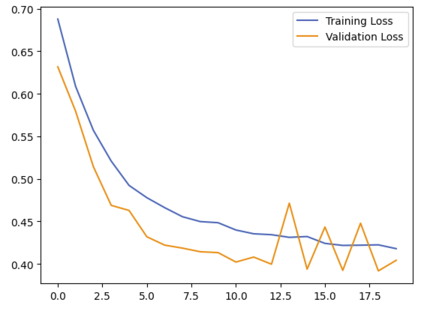
\includegraphics{picture1.png}
    \caption{trainingLoss / ValidationLoss}
    \label{fig:my_pic}
\end{figure}



\subsection{(10 Puan)} \textbf{SEED=öğrenci numaranız set ettikten sonra altıncı haftada ödev olarak verdiğim gibi earlystopping'deki en iyi modeli kullanarak, Prensesi İyileştir test setinden accuracy, F1, precision ve recall değerlerini hesaplayan kodu yazın ve sonucu da aşağı yapıştırın. \%80'den fazla başarı bekliyorum test setinden. Daha düşükse başarı oranınız, nerede hata yaptığınızı bulmaya çalışın. \%90'dan fazla başarı almak mümkün (ben denedim).}

\begin{python}
# Early stopping yapalım
best_val_acc = 0
patience = 3
counter = 0
for epoch in range(10):
    train(model, train_dataloader, optimizer, loss_fn)
    val_acc = evaluate(model, val_dataloader)
    print('Epoch:', epoch+1, '| Validation Accuracy:', val_acc)
    if val_acc > best_val_acc:
        best_val_acc = val_acc
        torch.save(model.state_dict(), 'best_model.pt')
        counter = 0
    else:
        counter += 1
        if counter >= patience:
            print('Early stopping.')
            break
            
# En iyi modeli yükleyelim
model.load_state_dict(torch.load('best_model.pt'))

# Test verisi üzerinde modelin doğruluğunu hesaplayalım
test_acc = evaluate(model, test_dataloader)
print('Test Accuracy:', test_acc)
# F1, Precision ve Recall değerlerini hesaplayalım
model.eval()
y_true = []
y_pred = []
with torch.no_grad():
    for data, target in test_dataloader:
        output = model(data)
        _, predicted = torch.max(output.data, 1)
        y_true += target.numpy().tolist()
        y_pred += predicted.numpy().tolist()
from sklearn.metrics import classification_report
target_names = ['not_cured', 'cured']
print(classification_report(y_true, y_pred, target_names=target_names))
\end{python}

\begin{minipage}[t]{0.5\textwidth}
    \centering
    \begin{tabular}{cc}
        Epoch: 1 & Validation Accuracy: 64.01\% \\
        Epoch: 2 & Validation Accuracy: 89.49\% \\
        Epoch: 3 & Validation Accuracy: 80.89\% \\
        Epoch: 4 & Validation Accuracy: 92.99\% \\
        Epoch: 5 & Validation Accuracy: 92.99\% \\
        Epoch: 6 & Validation Accuracy: 81.21\% \\
        Epoch: 7 & Validation Accuracy: 77.71\% \\
        & Early stopping. \\
        & Test Accuracy: 90.41\%
    \end{tabular}
\end{minipage}


\begin{table}[h]
    \centering
    \begin{minipage}[t]{0.5\textwidth}
        \centering
        \begin{tabular}{lccc}
            \hline
             & Precision & Recall & F1-Score \\ \hline
            not\_cured & 0.94 & 0.86 & 0.90 \\ \hline
            cured & 0.88 & 0.94 & 0.91 \\ \hline
            accuracy & \multicolumn{3}{c}{0.90} \\ \hline
            macro avg & 0.91 & 0.90 & 0.90 \\ \hline
            weighted avg & 0.91 & 0.90 & 0.90 \\ \hline
        \end{tabular}
        \caption{Classification Report}
        \label{tab:classification_report}
    \end{minipage}
\end{table}
\subsection{(5 Puan)} \textbf{Tüm kodların CPU'da çalışması ne kadar sürüyor hesaplayın. Sonra to device yöntemini kullanarak modeli ve verileri GPU'ya atıp kodu bir de böyle çalıştırın ve ne kadar sürdüğünü hesaplayın. Süreleri aşağıdaki tabloya koyun. GPU için Google Colab ya da Kaggle'ı kullanabilirsiniz, iki ortam da her hafta saatlerce GPU hakkı veriyor.}

\begin{table}[ht!]
    \centering
    \caption{Multilayer Perceptron (MLP) Saving The Princess_1}
    \begin{tabular}{c|c}
        Ortam & Süre (saniye) \\\hline
        CPU & 13.53 seconds. \\ 
        GPU & 1.17 seconds.\\
    \end{tabular}
    \label{tab:my_table}
\end{table}

\begin{table}[ht!]
    \centering
    \caption{Multilayer Perceptron (MLP) Saving The Princess_2}
    \begin{tabular}{c|c}
        Ortam & Süre (saniye) \\\hline
        CPU & 5.70 seconds. \\ 
        GPU & 1.15 seconds.\\
    \end{tabular}
    \label{tab:my_table}
\end{table}

\begin{table}[ht!]
    \centering
    \caption{Multilayer Perceptron (MLP) Saving The Princess_3}
    \begin{tabular}{c|c}
        Ortam & Süre (saniye) \\\hline
        CPU & 9.86 seconds. \\ 
        GPU & 1.23 seconds.\\
    \end{tabular}
    \label{tab:my_table}
\end{table}
\subsection{(3 Puan)} \textbf{Modelin eğitim setine overfit etmesi için elinizden geldiği kadar kodu gereken şekilde değiştirin, validasyon loss'unun açıkça yükselmeye başladığı, training ve validation loss'ları içeren figürü aşağı koyun ve overfit için yaptığınız değişiklikleri aşağı yazın. Overfit, tam bir çanak gibi olmalı ve yükselmeli. Ona göre parametrelerle oynayın.}

\begin{figure}[ht!]
    \centering
    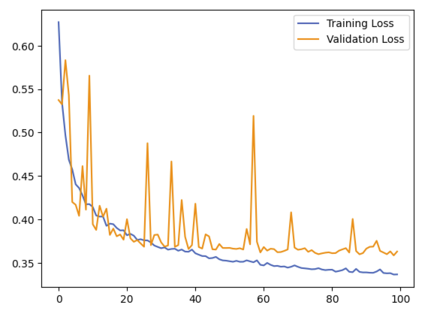
\includegraphics{picture2.png}
    \caption{trainingLoss / ValidationLoss}
    \label{fig:my_pic}
\end{figure}


\subsection{(2 Puan)} \textbf{Beşinci soruya ait tüm kodların ve cevapların olduğu jupyter notebook'un Github linkini aşağıdaki url'e koyun.}

\url{https://github.com/nazlicancay/Multilayer-Perceptron-MLP-Example} \\
\url{https://github.com/nazlicancay/Feed_Forward_example}

\section{(Toplam 10 Puan)} \textbf{Bir önceki sorudaki Prensesi İyileştir problemindeki yapay sinir ağınıza seçtiğiniz herhangi iki farklı regülarizasyon yöntemi ekleyin ve aşağıdaki soruları cevaplayın.} 

\subsection{(2 puan)} \textbf{Kodlarda regülarizasyon eklediğiniz kısımları aşağı koyun:} 


\begin{python}
# L2 Regülerizasyonu (Weight Decay):
In [24]:
class MLP(nn.Module):
    def __init__(self):
        super(MLP, self).__init__()
        self.fc1 = nn.Linear(13, 100)
        self.fc2 = nn.Linear(100, 50)
        self.fc3 = nn.Linear(50, 2)
        
    def forward(self, x):
        x = nn.functional.relu(self.fc1(x))
        x = nn.functional.relu(self.fc2(x))
        x = nn.functional.sigmoid(self.fc3(x))
        return x
    
# L2 Regülerizasyonu
l2_reg = 0.01
for param in model.parameters():
    param.data -= l2_reg * param.data.norm(2)

    # Dropout Regülerizasyonu

class MLP(nn.Module):
    def __init__(self):
        super(MLP, self).__init__()
        self.fc1 = nn.Linear(13, 100)
        self.dropout1 = nn.Dropout(p=0.5)
        self.fc2 = nn.Linear(100, 50)
        self.dropout2 = nn.Dropout(p=0.5)
        self.fc3 = nn.Linear(50, 2)
        
    def forward(self, x):
        x = nn.functional.relu(self.fc1(x))
        x = self.dropout1(x)
        x = nn.functional.relu(self.fc2(x))
        x = self.dropout2(x)
        x = nn.functional.sigmoid(self.fc3(x))
        return x

\end{python}

\subsection{(2 puan)} \textbf{Test setinden yeni accuracy, F1, precision ve recall değerlerini hesaplayıp aşağı koyun:}

# L2 Regülerizasyonu
Epoch: 1 | Validation Accuracy: 92.35668789808918 \\
Epoch: 2 | Validation Accuracy: 92.67515923566879 \\ 
Epoch: 3 | Validation Accuracy: 92.67515923566879 \\ 
Epoch: 4 | Validation Accuracy: 91.71974522292993 \\ 
Epoch: 5 | Validation Accuracy: 92.03821656050955 \\ 
Early stopping. \\ 
\\ 
Test Accuracy: 87.56476683937824\\ 
Test Precision: 0.8578431372549019\\ 
Test Recall: 0.9020618556701031\\ 
Test F1-score: 0.879396984924623\\ 

# Dropout Regülerizasyonu

Epoch: 1 | Validation Accuracy: (92.35668789808918 \\
Epoch: 2 | Validation Accuracy: (92.67515923566879 \\
Epoch: 3 | Validation Accuracy: (92.67515923566879 \\
Epoch: 4 | Validation Accuracy: (92.67515923566879  \\
Epoch: 5 | Validation Accuracy: (92.99363057324841  \\


Test Accuracy: 67.09844559585493 \\
Test Precision: 67.5535329451144 \\
Test Recall: 67.09844559585493 \\
Test F1: 66.85631294439585 \\



\subsection{(5 puan)} \textbf{Regülarizasyon yöntemi seçimlerinizin sebeplerini ve sonuçlara etkisini yorumlayın:}

regülasyon kullanmamaızın sebebi overfitting problemini önlemek ve genelleştirilebilirliği arttırmaktır. L1 ve L2 regülasyonları kullanarak modeldeki ağırlıkların büyüklüklerini sınırlandırmış  aşırı uyum sorununu engeller.

Dropout yöntemiyse ağdaki nöronların rastgele bir kısmının çıkışını 0'layarak (atma) bu nöronların çalışmamasını sağlar. 

bu regülasyonlar sayesinde modelin farklı bölümleri ayrı ayrı öğretilmiş olur. Bu da genelleştirilebilirliliği arttırır. Ancak, her yöntem her zaman her model ve veri kümesi için en iyi sonucu vermez. örneğin saveing the princess örneğinde dropout regülasyonu l2 regülasyonundan biraz daha  yüksek 

\subsection{(1 puan)} \textbf{Sonucun github linkini  aşağıya koyun:}


\url{https://github.com/nazlicancay/Multilayer-Perceptron-MLP-Example/blob/main/RegülationExample.ipynb}\\
\end{document}